\begin{frame}
	\begin{itemize}
	\item Objectif double~: 
		\begin{itemize}
		\item Vérifier la validité du programme écrit~;
		\item Générer un arbre abstrait analysable par l'analyseur sémantique.
		\end{itemize}
	\item Langage utilisé~: GNU Bison (Yacc).
	\end{itemize}
\end{frame}

\begin{frame}[fragile]
	\begin{rail}
		selection : IF expr statement \\ (ELSE statement) ? ;
	\end{rail}
\end{frame}

\begin{frame}
La partie haute de l'exemple précédent génère l'abre abstrait suivant~:
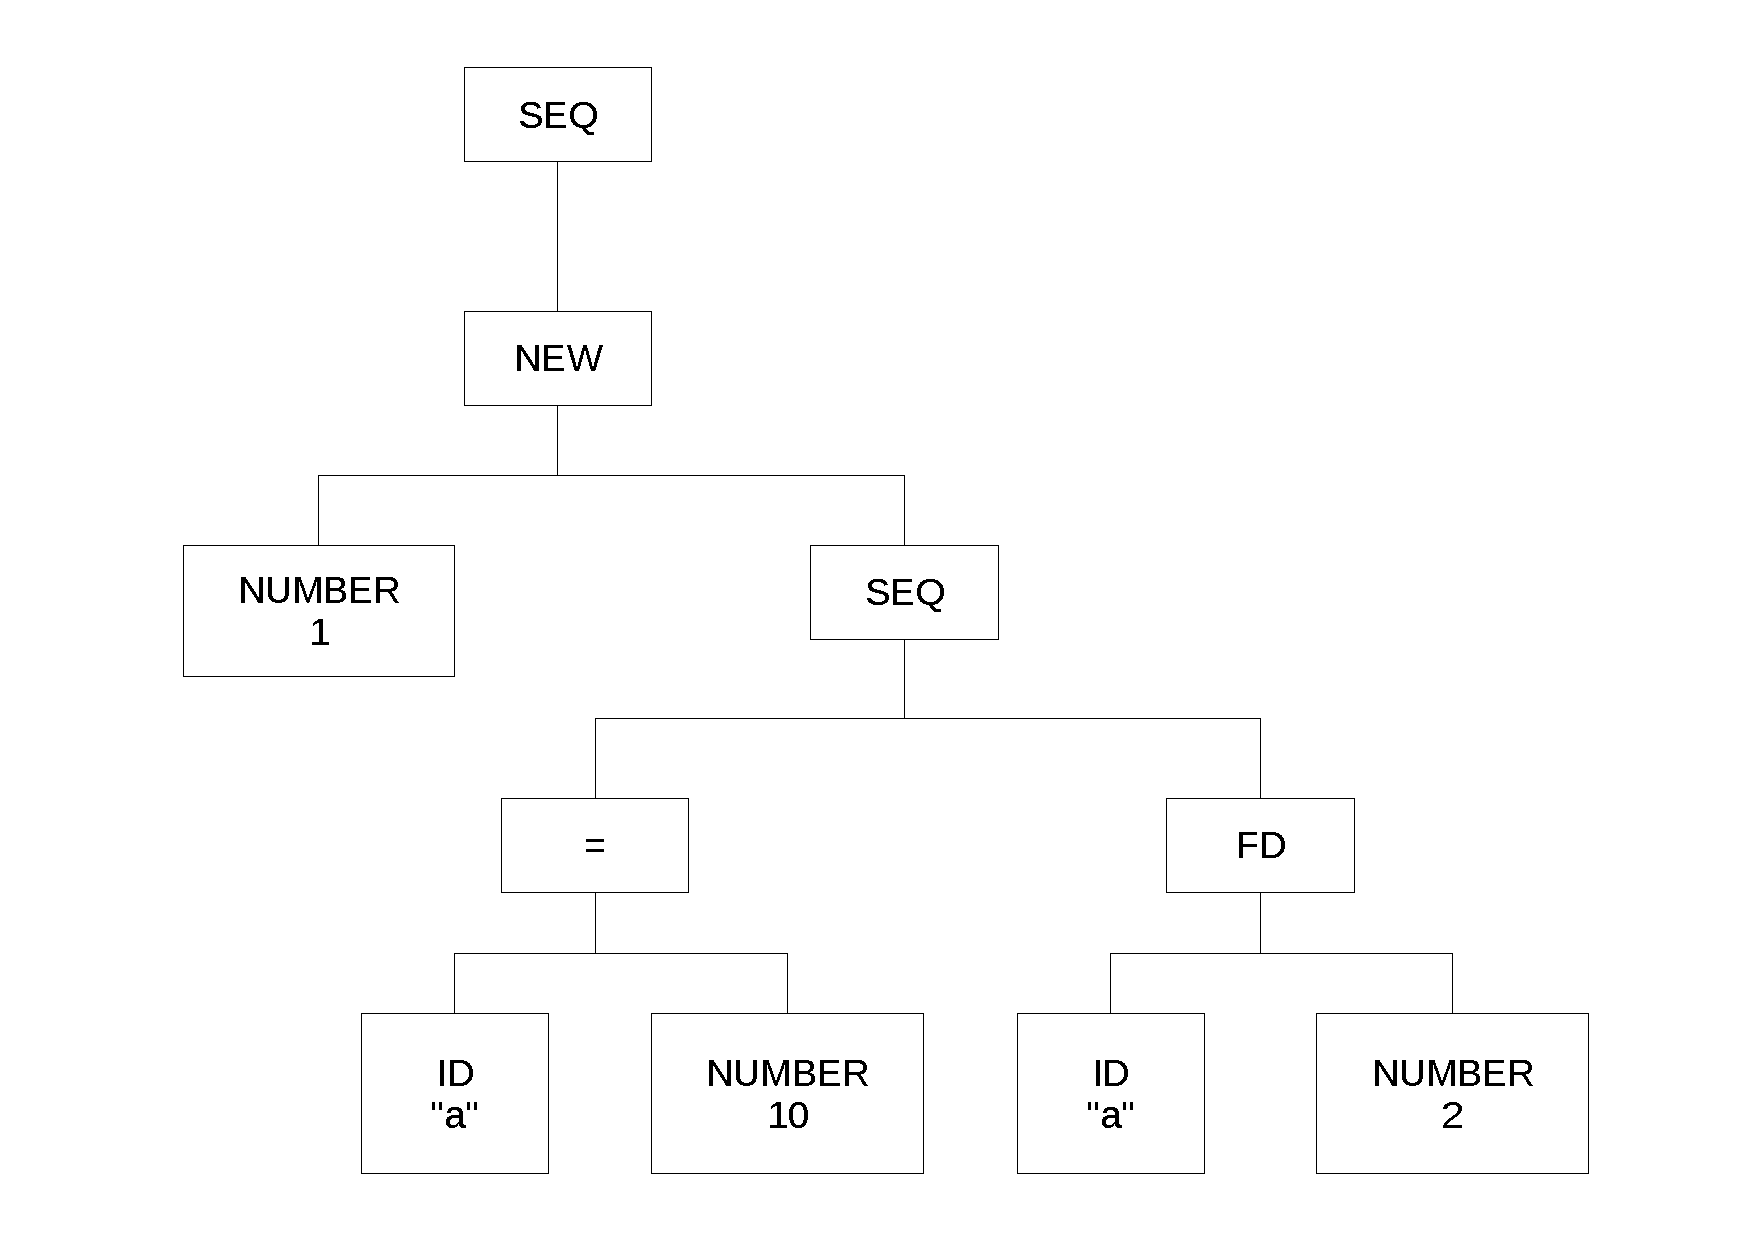
\includegraphics[scale=0.3]{doc/Presentation/img/arbre.pdf}
\end{frame}
